\documentclass[a4paper]{article} 
\usepackage{geometry}
\geometry{left=2.2cm,right=2.2cm,top=2.5cm,bottom=2.5cm}
\usepackage{ctex}       %载入中文包
\title{无线网络系统}
\author{高等理工学院\ 王冠楠}
\date{}
\begin{document}
\maketitle

\section{AODV介绍}
\subsection{AODV概述}
AODV全称为Ad hoc On-demand Distance Vector Routing,是为快速移动自组网(MANET)设计的数据包路由协议,较适用于有大量节点的无线自主网络。作为一种\textbf{按需路由协议},只有当到达某目的节点的路由不存在时才会激活该协议发起路由请求。使用节点序列号机制避免环路产生。传输层使用的是UDP协议。网络各节点使用IP地址统一编址。每一个节点维护一个包含到达目的节点路由信息的路由表。

当一个节点需要给网络中的其他节点传送信息时,如果没有到达目标节点的路由,则必须先以\textbf{多播}的形式发出\textbf{RREQ(路由请求)}报文。RREQ报文中记录着发起节点和目标节点的网络层地址,邻近节点收到RREQ,首先判断目标节点是否为自己。如果是,则向发起节点发送\textbf{RREP(路由回应)};如果不是,则首先在路由表中查找是否有到达目标节点的路由,如果有,则向源节点单播RREP,否则继续转发RREQ进行查找。
\begin{figure}[htbp]
	\centering
	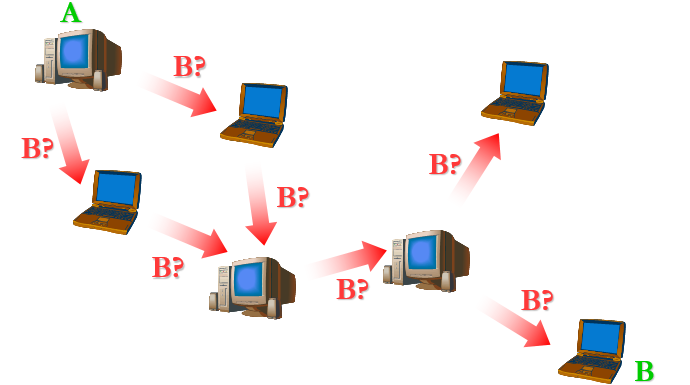
\includegraphics[width=8cm]{1.png}
	\caption{RREQ请求帧传播}
\end{figure}
\begin{figure}[htbp]
	\centering
	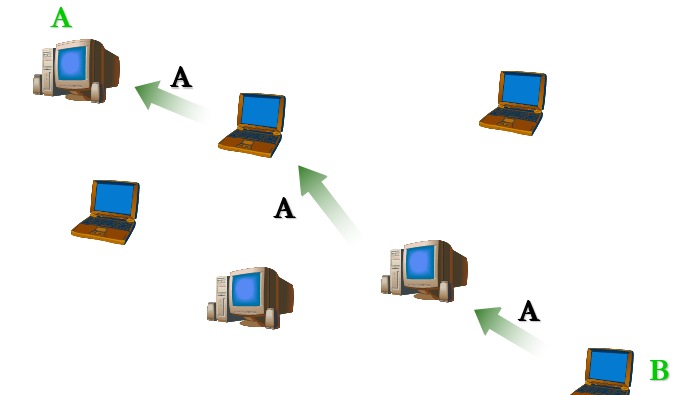
\includegraphics[width=8cm]{2.png}
	\caption{RREP应答帧传播}
\end{figure}

\subsubsection{路由表字段}
路由表字段由以下部分组成:

1.目的节点IP地址

2.目的节点序列号(Sequence Number)

3.目的节点序列号有效标志位

4.下一跳节点IP地址

5.本节点到达目的节点的跳数

6.前驱节点列表(precursor list)

7.生存时间(路由失效或删除时间)

8.网络层接口

9.其他的状态和路由标志位

路由表每项只记录下一跳路由信息,而不是整条路由信息,简化了路由表的建立和维护。源节点和目的节点都维护各自的序列号。如何管理序列号是提高路由建立和维护的关键。序列号是用来标识路由信息新旧程度(freshness)的。源节点发起路由请求RREQ,或者目的节点返回路由应答RREP,都要更新各自的序列号。其他节点(中间节点)依据序列号的大小判断路由的新旧。
\subsection{AODV路由帧}
AODV路由帧格式主要包括:

1.RREQ\ –\ 路由请求帧

2.RREP\ –\ 路由应答帧

3.RERR\ –\ 路由错误帧

4.HELLO\ –\ 活跃路由链路监测帧
\begin{figure}[htbp]
	\centering
	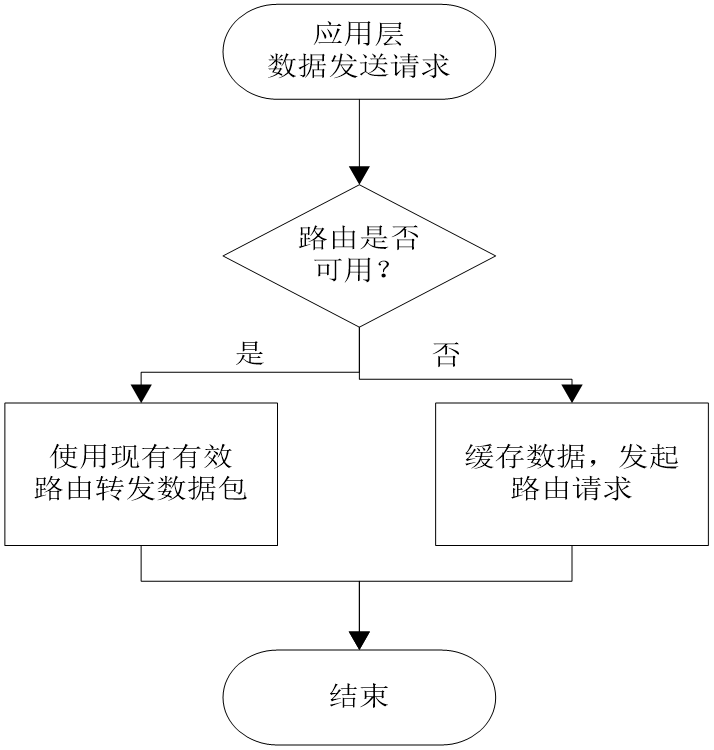
\includegraphics[width=8cm]{3.png}
	\caption{AODV路由请求的发起流程图}
\end{figure}
\begin{figure}[htbp]
	\centering
	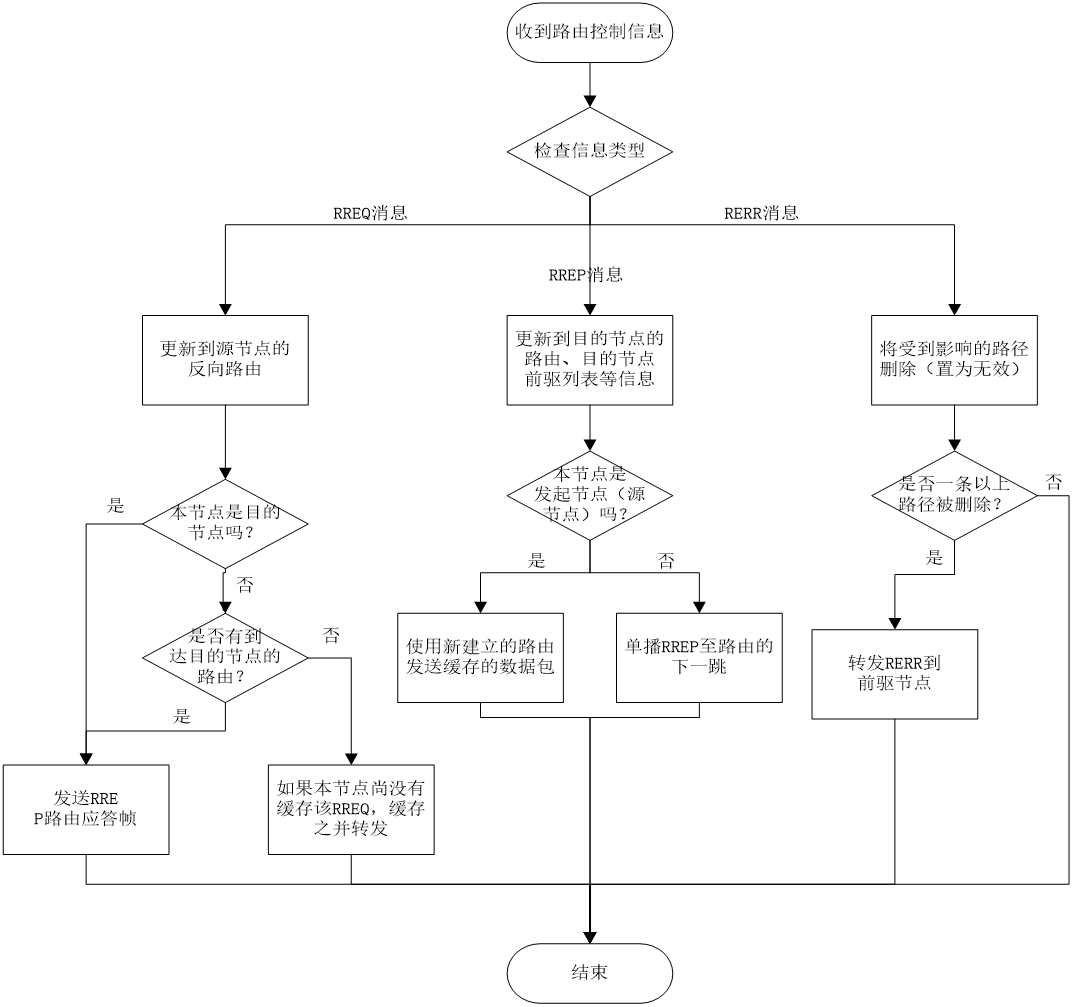
\includegraphics[width=14cm]{4.png}
	\caption{AODV对路由控制信息的控制流程图}
\end{figure}
\newpage
\subsubsection{路由请求帧RREQ}
\begin{figure}[htbp]
	\centering
	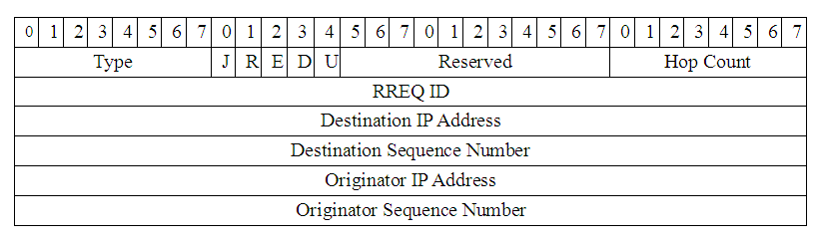
\includegraphics[width=14cm]{5.png}
	\caption{RREQ路由请求帧}
\end{figure}
\subsubsection{路由应答帧RREP}
\subsubsection{路由错误帧RRRR}
\subsubsection{活跃路由链路监测帧HELLO}
\section*{参考}
https://wenku.baidu.com/browse/downloadrec?doc\_id=6ca1b900de80d4d8d15a4ff6\&

\end{document}

%\section{第一部分}
%写点什么吧。
%\subsection{第一部分的二小部分}
%say hello.
%
%\section*{第二部分}
%再写点什么吧。